\documentclass[serif, aspectratio=169]{beamer}
\usepackage[T1]{fontenc} 
\usepackage{fourier}
\usepackage{hyperref}
\usepackage{latexsym,amsmath,xcolor,multicol,booktabs,calligra}
\usepackage{booktabs} % For better table formatting
\usepackage{graphicx,pstricks,listings,stackengine}
\usepackage{listings}
\usepackage{array} 
\usepackage{colortbl}

\author{Dr.Hajialiasgari}
\title{Machine Learning}
\institute{
    Tehran University \\
    Of\\
    Medical Science
}
\date{\small \today}
\usepackage{UoWstyle}

% Define custom colors and styles for listings
\definecolor{deepblue}{rgb}{0,0,0.5}
\definecolor{deepred}{RGB}{153,0,0}
\definecolor{deepgreen}{rgb}{0,0.5,0}
\definecolor{halfgray}{gray}{0.55}

\lstset{
    basicstyle=\ttfamily\small,
    keywordstyle=\bfseries\color{deepblue},
    emphstyle=\ttfamily\color{deepred},
    stringstyle=\color{deepgreen},
    numbers=left,
    numberstyle=\small\color{halfgray},
    rulesepcolor=\color{red!20!green!20!blue!20},
    frame=shadowbox,
}

\begin{document}

\begin{frame}
    \titlepage
    \vspace*{-0.6cm}
    \begin{figure}[htpb]
        \begin{center}
            \includegraphics[keepaspectratio, scale=0.05]{Tumsl-logo.png}
        \end{center}
    \end{figure}
\end{frame}

\begin{frame}    
\tableofcontents[sectionstyle=show, subsectionstyle=show/shaded/hide, subsubsectionstyle=show/shaded/hide]
\end{frame}

\section{Decision Tree}
\begin{frame}{Overview of Decision Trees}
    \begin{itemize}
        \item Decision Trees are used for both classification and regression.
        \item They split data into branches based on feature values.
        \item The tree consists of \textbf{nodes} (decisions) and \textbf{leaves} (predictions).
    \end{itemize}
\end{frame}

\begin{frame}{Decision Tree (Cont.)}
    \centering
    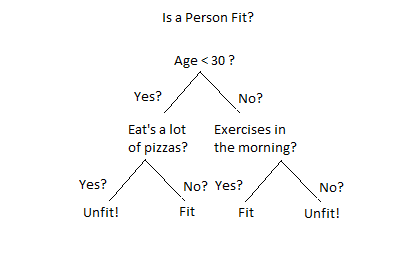
\includegraphics[width=0.9\textwidth]{Decision-Trees-modified-1.png}
\end{frame}

\begin{frame}{How Decision Trees Work}
    \begin{itemize}
        \item Starts with the entire dataset at the root.
        \item Splits the dataset based on a selected feature using a splitting criterion (e.g., Gini Impurity, Entropy, or Mean Squared Error).
        \item Repeats the process recursively until stopping criteria are met (e.g., max depth, minimum samples per leaf).
        \item Outputs a final prediction based on leaf nodes.
    \end{itemize}
\end{frame}

\begin{frame}{Decision Tree Structure}
    \centering
    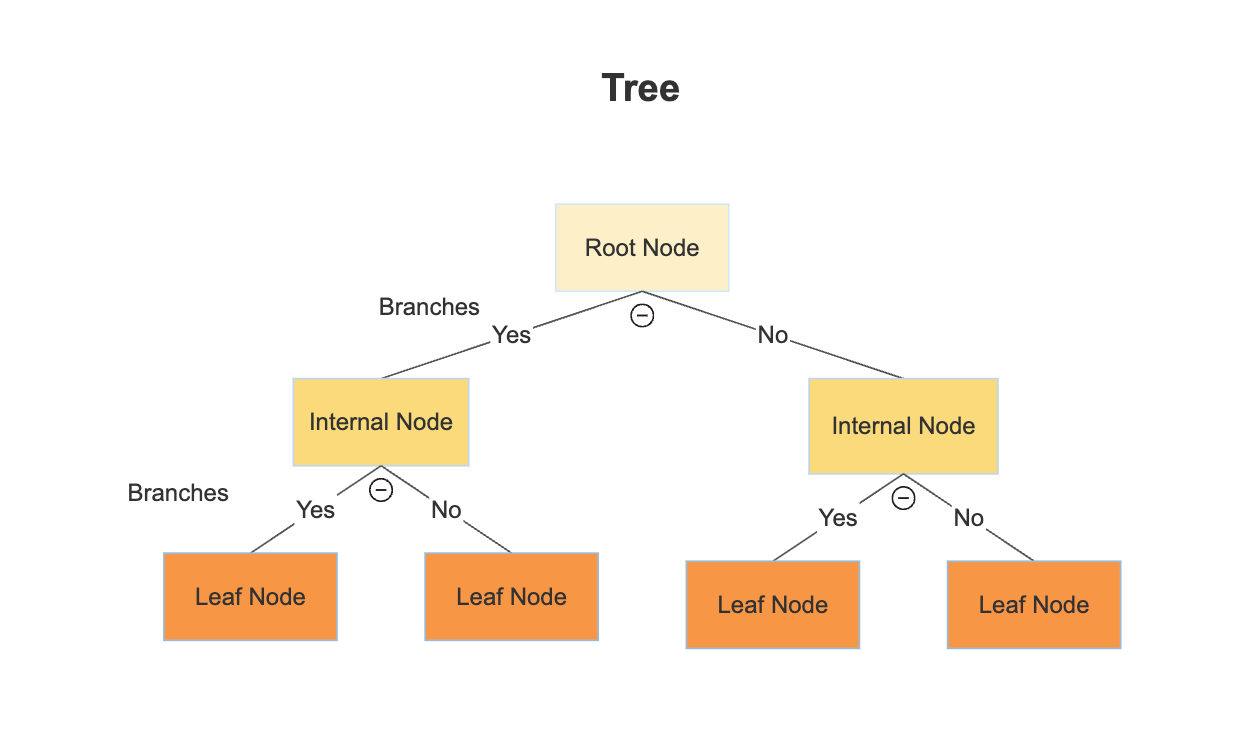
\includegraphics[width=0.9\textwidth]{Decision_Tree_2.png}
\end{frame}

% Slide 3: Splitting Criteria
\begin{frame}{Splitting Criteria (1)}
    \textbf{1. Gini Impurity:}
    \begin{equation}
        Gini = 1 - \sum_{i=1}^{C} p_i^2
    \end{equation}
    \textbf{2. Entropy:}
    \begin{equation}
        Entropy = - \sum_{i=1}^{C} p_i \log_2 p_i
    \end{equation}
\end{frame}

\begin{frame}{Splitting Criteria (Cont.)}
    \textbf{3. Information Gain:}
    \begin{equation}
        IG = Entropy(parent) - \sum_{i} \frac{|subset_i|}{|parent|} \times Entropy(subset_i)
    \end{equation}
    \textbf{4. Mean Squared Error (for Regression):}
    \begin{equation}
        MSE = \frac{1}{N} \sum_{i=1}^{N} (y_i - \hat{y}_i)^2
    \end{equation}
\end{frame}


\begin{frame}{Example}
    \centering
    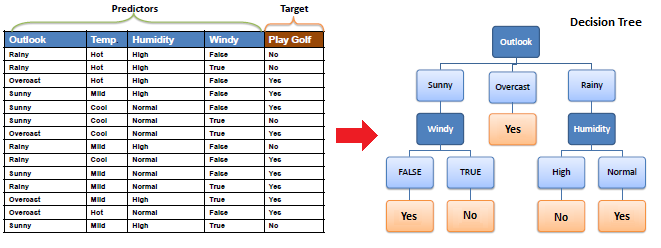
\includegraphics[width=0.9\textwidth]{Decision_Tree_1.png}
\end{frame}

% Slide 4: Medical Example
\begin{frame}{Example: Medical Diagnosis}
    \begin{itemize}
        \item Features: Age, Cholesterol, Blood Pressure, Smoking Status.
        \item Example Rule: 
        \begin{itemize}
            \item If Cholesterol > 240 and Blood Pressure > 140, classify as High Risk.
            \item Else, classify as Low Risk.
        \end{itemize}
    \end{itemize}
\end{frame}

% Slide 5: Insurance Example
\begin{frame}{Example: Insurance Risk Prediction}
    \begin{itemize}
        \item Features: Age, Driving History, Number of Accidents, Type of Car.
        \item Example Rule:
        \begin{itemize}
            \item If Age < 25 and Accidents > 2, classify as High Risk.
            \item If Age >= 25 and No Accidents, classify as Low Risk.
        \end{itemize}
    \end{itemize}
\end{frame}

% Slide 6: Advantages
\begin{frame}{Advantages of Decision Trees}
    \begin{itemize}
        \item Easy to interpret and visualize.
        \item Handles both numerical and categorical data.
        \item Requires little data preprocessing.
        \item Works well with large datasets.
    \end{itemize}
\end{frame}

% Slide 7: Disadvantages
\begin{frame}{Disadvantages of Decision Trees}
    \begin{itemize}
        \item Can overfit the data (prone to high variance).
        \item Sensitive to noisy data.
        \item Can create biased results if dataset is imbalanced.
    \end{itemize}
\end{frame}

% Slide 8: Improving Decision Trees
\begin{frame}{Improving Decision Trees}
    \begin{itemize}
        \item \textbf{Pruning:} Reducing tree size to avoid overfitting.
        \item \textbf{Ensemble Methods:} Combining multiple trees (Random Forest, Gradient Boosting).
        \item \textbf{Feature Selection:} Choosing relevant features improves accuracy.
    \end{itemize}
\end{frame}

\section{Overfitting in Decision Tree}

\begin{frame}{Overview}
    \textbf{Definition:} Overfitting occurs when a decision tree learns patterns specific to the training data but fails to generalize to unseen data.
    \begin{itemize}
        \item The tree becomes too complex and captures noise instead of the true pattern.
        \item Leads to high accuracy on training data but poor performance on test data.
    \end{itemize}
    \textbf{Causes of Overfitting:}
    \begin{itemize}
        \item Deep trees with too many splits.
        \item Small leaf nodes capturing noise.
        \item High variance in data leading to unstable decision boundaries.
    \end{itemize}
\end{frame}

% Slide: Preventing Overfitting
\begin{frame}{Preventing Overfitting in Decision Trees}
    \textbf{1. Pruning}
    \begin{itemize}
        \item \textbf{Pre-pruning (Early Stopping):} Stop tree growth based on depth or information gain threshold.
        \item \textbf{Post-pruning:} Grow the full tree, then remove branches that do not improve validation accuracy.
    \end{itemize}
    \textbf{2. Restricting Tree Growth}
    \begin{itemize}
        \item Limit maximum depth of the tree.
        \item Require a minimum number of samples per leaf node.
        \item Set a minimum number of samples needed to split a node.
    \end{itemize}
\end{frame}


\begin{frame}{A Pruned Tree}
    \centering
    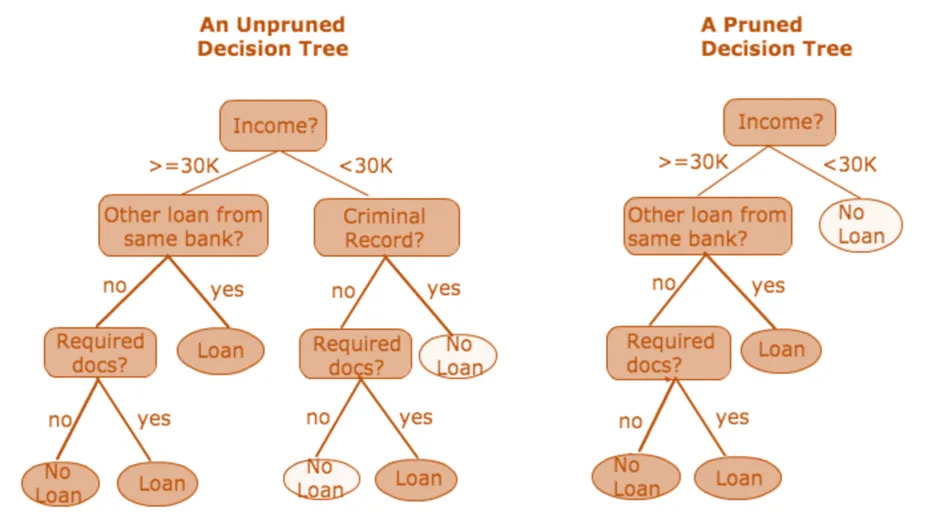
\includegraphics[width=0.9\textwidth]{A_Pruned_Tree.jpg}
\end{frame}

% Slide: Advanced Techniques
\begin{frame}{Advanced Techniques to Control Overfitting}
    \textbf{3. Ensemble Methods}
    \begin{itemize}
        \item \textbf{Random Forests:} Combine multiple trees and average predictions to reduce variance.
        \item \textbf{Boosting (e.g., AdaBoost, Gradient Boosting):} Train sequential trees that correct previous errors.
    \end{itemize}
    \textbf{4. Regularization Techniques}
    \begin{itemize}
        \item \textbf{Cost Complexity Pruning (CCP):} Penalizes complex trees by adding a cost term for additional nodes.
    \end{itemize}
\end{frame}

\begin{frame}
    \begin{center}
        {\Huge\ \color{red}For more information and code check the related notebook}
    \end{center}
\end{frame}


\begin{frame}
    \begin{center}
        {\Huge\ End of Classification}
    \end{center}
\end{frame}

\end{document}

